\Chapter{LITERATURE REVIEW}\label{sec:RevLitt}


This chapter reviews the main numerical ingredients involved in aircraft ice accretion simulations. The first section focuses on water-droplet tracking techniques, with particular attention to Eulerian and Lagrangian formulations used to predict droplet impingement. The second section discusses Supercooled Large Droplet (SLD) effects and the semi-empirical models commonly used to account for splashing, bouncing, and secondary droplet behavior. The final sections review immersed-boundary methods, surface-representation techniques, and wall-function approaches relevant to robust ice accretion simulations.

\section{Water-Droplet Tracking}

Water-droplet tracking is a central component of aircraft icing simulations. Before ice growth can be computed, the locations and rates at which droplets impinge on the aircraft surface must be determined. This impingement distribution directly affects the local water mass flux, the surface thermodynamic balance, and ultimately the predicted ice shape. Over the past decades, several numerical methods have been developed to model droplet transport in icing conditions. These methods generally seek a balance between accuracy, computational cost, robustness, and ease of integration into existing flow solvers.

Two main families of approaches are commonly used in the literature: Eulerian and Lagrangian methods. Eulerian models treat the droplet phase as a continuous medium. Governing equations similar to those used for the airflow are solved to obtain the droplet velocity field and the local water concentration throughout the computational domain. This formulation offers several advantages. It is generally computationally efficient, naturally suited for parallelization, and relatively easy to integrate into a finite-volume flow-solver framework. However, Eulerian methods also present limitations. Since the droplet phase is represented as a continuum, individual droplet information is lost, and phenomena such as splashing, breakup, and secondary droplet motion are more difficult to model directly. In addition, artificial dissipation and numerical oscillations can affect the solution, sometimes leading to nonphysical values such as negative water concentration. Such issues must be treated carefully, especially for complex geometries such as multi-element airfoils. Several techniques have been proposed to improve the robustness and conservation properties of Eulerian droplet solvers \cite{blanchet2022conservative}.

Lagrangian methods, on the other hand, track droplets or droplet parcels individually by solving their equations of motion along their trajectories. Historically, these methods were limited by their computational cost, especially when a large number of droplets was required to obtain smooth impingement maps. However, advances in high-performance computing have renewed interest in Lagrangian approaches for aircraft icing applications. These methods naturally provide access to individual droplet trajectories, impact velocities, and impact angles, which makes them particularly attractive for studying SLD effects and droplet-wall interactions.

The choice between Eulerian and Lagrangian droplet tracking therefore depends on the targeted application and on the acceptable trade-off between computational efficiency, accuracy, and physical detail.

\subsection{Eulerian Droplet Tracking}\label{sec:eulerianTracking}

Eulerian dispersed-phase tracking is based on a system of partial differential equations describing the evolution of the droplet concentration and droplet momentum. This formulation was first introduced for aircraft icing applications by Bourgault et al. \cite{bourgault1999finite}. The continuity equation is solved to obtain the nondimensional water concentration $\alpha$:

\begin{equation}
\frac{\partial \alpha}{\partial t} + \nabla \cdot (\alpha \boldsymbol{u_d}) = 0 ,
\label{eq: continuityDroplet}
\end{equation}

where $\boldsymbol{u_d}$ is the droplet velocity. The corresponding momentum equation provides the droplet velocity field:

\begin{equation}
\frac{\partial (\alpha \boldsymbol{u_d})}{\partial t} +  \nabla \cdot (\alpha \boldsymbol{u_d} \otimes \boldsymbol{u_d}) = \frac{C_D , Re_D}{24K} \alpha (\boldsymbol{u_a} - \boldsymbol{u_d}) + \alpha \left(1-\frac{\rho_a}{\rho_w}\right) \frac{\boldsymbol{g}}{Fr^2}.
\label{eq: momentumDroplet}
\end{equation}

In this model, only drag and gravity forces are considered. The first term on the right-hand side of Equation~\ref{eq: momentumDroplet} represents the aerodynamic drag exerted by the airflow of velocity $\boldsymbol{u_a}$ on the droplet phase. The second term accounts for gravity.

Eulerian droplet tracking offers several advantages. It is computationally efficient because individual droplets are not tracked separately. It is also well suited for high-performance computing, since the numerical structure of the droplet equations is similar to that of the airflow equations. This similarity facilitates implementation in existing finite-volume solvers and allows the same parallelization strategy to be reused.

However, the Eulerian formulation also has important limitations. Since the droplet phase is averaged over the computational cells, individual droplet trajectories are not directly available. Microscale phenomena, such as droplet splashing, bouncing, and breakup, are difficult to represent without additional models. Numerical diffusion may also smear the impingement limits and reduce the accuracy of the local collection efficiency. Finally, for low droplet volume fractions or complex configurations, the dispersed phase may be poorly resolved, leading to nonphysical oscillations or negative values of the water concentration.

\subsection{Lagrangian Droplet Tracking}\label{sec:LagDropTracking}

In a Lagrangian formulation, droplets or droplet parcels are tracked by integrating their equation of motion. The droplet velocity $\boldsymbol{u_d}$ is first computed, and the droplet position is then obtained through an additional integration step. The equation of motion can be written as

\begin{equation}
\frac{d\boldsymbol{u_d}}{dt} = \frac{\boldsymbol{f}}{m} + \boldsymbol{g} = F( \boldsymbol{u_a}- \boldsymbol{u_d}) + \boldsymbol{g},
\label{eq:eqOfMotion}
\end{equation}

where $\boldsymbol{f}$ is the aerodynamic force acting on the droplet, $m$ is the droplet mass, $\boldsymbol{g}$ is the gravitational acceleration, and $F$ is a scalar coefficient associated with drag.

The main assumptions used in the present Lagrangian formulation are as follows:

\begin{itemize}
\item The droplet mass remains constant before impact;
\item Droplets are independent from one another;
\item The droplet concentration is sufficiently low that the dispersed phase does not affect the airflow;
\item Turbulence effects on the droplet trajectories are neglected;
\item Droplet rotation and lift forces are neglected.
\end{itemize}

Under these assumptions, the only forces considered are aerodynamic drag and gravity. The scalar coefficient $F$ is obtained from the local droplet Reynolds number, based on the relative velocity $| \boldsymbol{u_a} - \boldsymbol{u_d} |$ and droplet diameter. This gives

\begin{equation}
F = \frac{C_D \frac{1}{2} \rho_a | \boldsymbol{u_a} -  \boldsymbol{u_d}| ^2 A}{m | \boldsymbol{u_a} -  \boldsymbol{u_d}|} = \frac{3 C_D  \rho_a | \boldsymbol{u_a} -  \boldsymbol{u_d}| }{4 \rho_w D},
\label{eq:forceCoef}
\end{equation}

where $C_D$ is the droplet drag coefficient, $\rho_a$ is the air density, $\rho_w$ is the water density, and $D$ is the droplet diameter.

A detailed analysis of numerical schemes for ordinary differential equations is presented by Darmofal and Haimes \cite{darmofal1996analysis}. Multistep schemes, such as Adams-Bashforth methods, and multistage schemes, such as Runge-Kutta methods, can be used to integrate droplet trajectories. However, particle-path integration may become unstable if the time step is too large. Therefore, a compromise must be found between computational cost, accuracy, and stability.

In aircraft icing applications, the trajectory integration also depends strongly on interpolation of the airflow velocity. Since droplet paths do not generally coincide with the computational mesh, the host cell of each droplet must be identified after each integration step. Several localization and tracking techniques have been proposed for this purpose.

\begin{figure}[htp]
\centering
\subfloat[Vicinity face-to-face tracking \cite{bellosta2023lagrangian}]{%
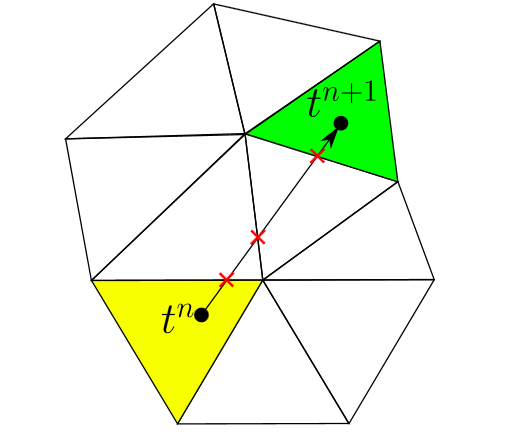
\includegraphics[width=0.25\textwidth]{FIGURES/Droplet_Tracking/vicinity.png}%
\label{fig:vicinity}%
}%
\hspace{1cm}%
\subfloat[Auxiliary-grid tracking \cite{li2019fast}]{%
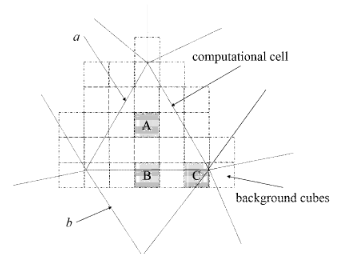
\includegraphics[width=0.31\textwidth]{FIGURES/Droplet_Tracking/supportGrid.png}%
\label{fig:auxGrid}%
}%
\hspace{1cm}%
\subfloat[Face-to-face tracking \cite{rendall2014finite}]{%
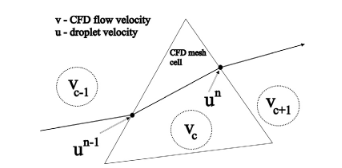
\includegraphics[width=0.31\textwidth]{FIGURES/Droplet_Tracking/faceTracking.png}%
\label{fig:faceTracking}%
}%
\caption{Examples of droplet-tracking techniques.}
\label{fig:dropletTracking}
\end{figure}

Tree-based search methods use octree-type data structures to identify the cell containing each droplet. Although general, these methods can become expensive for large-scale three-dimensional simulations. For example, a swept-wing dispersed-phase simulation may require several million droplets to obtain a sufficiently resolved impingement distribution. In this context, computational cost and parallel scalability are critical, which limits the practical use of global tree-based searches.

Known-vicinity face-to-face methods \cite{bellosta2023lagrangian} use the previous droplet location to identify the current host cell. After the droplet position is advanced, a ray is cast along the droplet trajectory. If the trajectory remains within the current cell, the host cell is unchanged. Otherwise, the droplet crosses a face into an adjacent cell, which is identified using mesh connectivity. This procedure is repeated until the final host cell is found. This approach avoids global searches and is therefore more efficient for large unstructured grids.

Auxiliary-grid methods \cite{li2019fast} use a structured background grid, typically Cartesian, to accelerate droplet localization. Before the simulation, a mapping is established between the background grid and the computational mesh. Each background cell stores the computational cells that it overlaps. During tracking, the droplet is first located in the auxiliary grid, and point-in-cell tests are then performed only on a small set of candidate computational cells. This can significantly reduce the cost of particle localization. However, the construction and storage of the background-grid mapping introduce additional preprocessing complexity, especially in three-dimensional simulations.

Face-to-face tracking \cite{rendall2014finite} provides an attractive compromise between efficiency and accuracy. The method relies directly on mesh connectivity. At each step, the droplet velocity defines a trajectory segment, and the next cell is identified by finding the nearest face intersection. The local time step is then obtained from the residence time of the droplet in the current cell. This approach avoids explicit global cell searches and is naturally compatible with finite-volume data structures. It is therefore well suited for large-scale unstructured simulations.

Because stability is a significant concern in droplet trajectory integration, implicit schemes are often preferred. Backward differentiation formulas provide an efficient and robust option \cite{rendall2014finite}. Further details on the implementation used in the present work are provided in Chapter~\ref{sec:RP}.

Using a first-order backward difference formula, the discretized equation of motion can be written as

\begin{equation}
\alpha m \boldsymbol{u_d}^n + \beta m \boldsymbol{u_d}^{n-1} = \boldsymbol{f}(\boldsymbol{u_a},\boldsymbol{u_d}) + m \boldsymbol{g} = m F (\boldsymbol{u_a}-\boldsymbol{u_d}) + m \boldsymbol{g},
\label{eq:BDF1}
\end{equation}

where $\alpha = 1/\Delta t$ and $\beta = -1/\Delta t$. The droplet velocity at the new time level is then obtained from

\begin{equation}
\boldsymbol{u_d}^{n} = \frac{ F \boldsymbol{u_a} -\beta \boldsymbol{u_d}^{n-1} +\boldsymbol{g}}{\alpha + F}.
\label{eq:BDF1_Time}
\end{equation}

A second-order formulation can be obtained by retaining the velocity from the previous two time levels:

\begin{equation}
\boldsymbol{u_d}^{n} = \frac{ F \boldsymbol{u_a} -\beta \boldsymbol{u_d}^{n-1}  -\gamma \boldsymbol{u_d}^{n-2} +\boldsymbol{g}}{\alpha + F}.
\label{eq:BDF2_Time}
\end{equation}

For variable time steps, the coefficients $\alpha$, $\beta$, and $\gamma$ are computed using the current time step $\Delta t_c$ and the previous time step $\Delta t_{c-1}$:

\begin{equation}
\alpha = \frac{2\Delta t_c+\Delta t_{c-1}}{(\Delta t_c+\Delta t_{c-1})\Delta t_c},
\label{eq:alpha}
\end{equation}

\begin{equation}
\beta = \frac{-(\Delta t_c+\Delta t_{c-1})}{\Delta t_c\Delta t_{c-1}},
\label{eq:beta}
\end{equation}

\begin{equation}
\gamma = \frac{\Delta t_c}{(\Delta t_c+\Delta t_{c-1})\Delta t_{c-1}}.
\label{eq:gamma}
\end{equation}

The trajectory integration is performed iteratively. An initial estimate of the new droplet velocity is obtained from the previous value, $\boldsymbol{u_d}^{n}=\boldsymbol{u_d}^{n-1}$. The airflow velocity at the new position is then estimated, and the nearest face intersection is computed using the current trajectory estimate. This provides the local time step and the corresponding coefficients in Equations~\ref{eq:alpha}–\ref{eq:gamma}. Equation~\ref{eq:BDF1_Time} or Equation~\ref{eq:BDF2_Time} is then used to update the droplet velocity. The process is repeated until the change between successive velocity estimates becomes sufficiently small.

The face intersection is computed using the midpoint velocity

\begin{equation}
\boldsymbol{u_d}^{n-\frac{1}{2}} = \frac{1}{2} \left(\boldsymbol{u_d}^n + \boldsymbol{u_d}^{n-1}\right).
\end{equation}

Because the local time step may vary significantly from one cell to another, the method may locally reduce to first-order accuracy. To mitigate this issue, limited gradients can be used to interpolate the airflow velocity at the droplet position:

\begin{equation}
\boldsymbol{u_a}{facet} = \boldsymbol{u_a}{cell} + \nabla \boldsymbol{u_a} \cdot \boldsymbol{d},
\label{eq:facetFlow}
\end{equation}

where $\boldsymbol{d}$ is the vector from the cell center to the droplet position.

The limiting behavior of Equation~\ref{eq:forceCoef} provides useful validation cases. For an infinitesimally small droplet, the coefficient $F$ tends to infinity, and the droplet velocity approaches the airflow velocity, $\boldsymbol{u_d}^{n} \approx \boldsymbol{u_a}^{n}$. In this limit, droplet trajectories coincide with airflow streamlines. Conversely, for very large droplets, $F$ tends toward zero, and the airflow has little influence on the droplet motion. The trajectory is then mainly governed by inertia and gravity.

\subsection{Collection Efficiency}\label{sec:CollEfficiency}

In addition to impingement locations, droplet tracking provides the collection efficiency of the geometry. The collection efficiency $\beta$ is a nondimensional measure of the local impingement rate. It relates the amount of water captured by a surface region to the amount of water that would pass through the corresponding upstream area, as illustrated in Figure~\ref{fig:collectionEfficiency}:

\begin{equation}
\beta = \frac{A_{upstream}}{A_{impingement}}.
\label{eq:betaEq}
\end{equation}

\begin{figure}[htp]
\centering
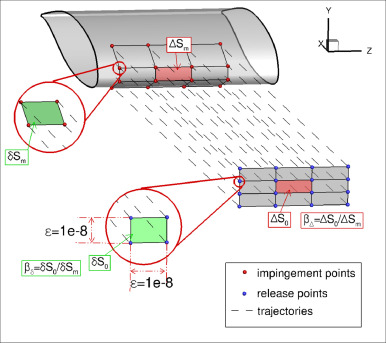
\includegraphics[trim={0.1cm 0.1cm 0.1cm 0.1cm},clip,width=.4\textwidth]{FIGURES/SLD/collectionEfficiency.jpg}
\caption{Computation of the collection efficiency from droplet trajectories \cite{xie2020robust}.}
\label{fig:collectionEfficiency}
\end{figure}

The collection efficiency is a key quantity in ice accretion simulations because it determines the incoming water mass flux on the surface. In Eulerian models, $\beta$ is obtained directly from the normal component of the droplet flux at the wall:

\begin{equation}
\beta = -\boldsymbol{u_d} \cdot \boldsymbol{\hat{n}},
\label{eq:betaEul}
\end{equation}

where $\boldsymbol{\hat{n}}$ is the outward unit normal to the surface.

In Lagrangian models, the computation of $\beta$ is more involved. A classical approach consists in tracking neighboring droplets and computing the ratio between the upstream seeding area and the corresponding impingement area. In two-dimensional simulations, this can be done using two neighboring trajectories. In three-dimensional simulations, three or four neighboring trajectories are generally required. However, this strategy introduces several difficulties.

First, in a parallel computing environment, neighboring droplets may be stored on different processors. Computing the local impingement area then requires additional communication, which may become expensive and difficult to manage. Second, neighboring droplets may not always impinge on the same component of a complex geometry. For example, in a multi-element airfoil, one droplet may impact the main element while another impacts the flap or slat, as shown in Figure~\ref{fig:collectionEfficiencyMDA}. In such cases, defining a meaningful local impingement area becomes ambiguous.

\begin{figure}[htp]
\centering
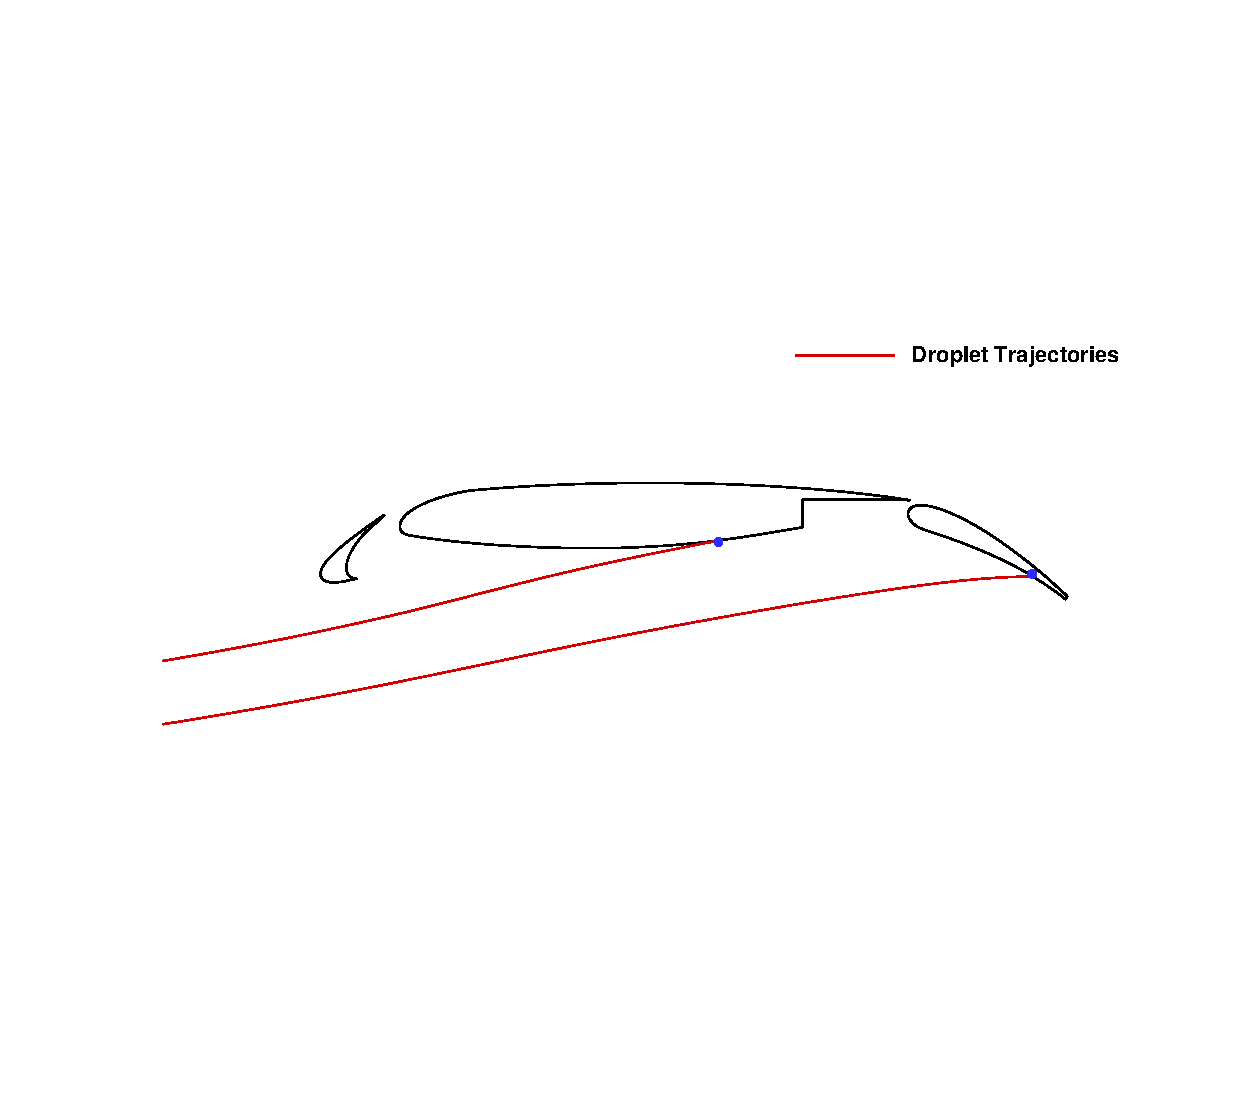
\includegraphics[trim={5cm 5cm 2cm 5cm},clip,width=.5\textwidth]{FIGURES/SLD/MDA.pdf}
\caption{Pathological case for collection-efficiency computation on a multi-element airfoil.}
\label{fig:collectionEfficiencyMDA}
\end{figure}

To address these issues, Xie et al. \cite{xie2020robust} proposed computing additional secondary trajectories around each primary droplet. Since the secondary trajectories are generated locally, they can be stored on the same processor, reducing communication requirements. The droplets are also released very close to one another, which increases the probability that they impinge on the same component of the geometry.

\section{Supercooled Large Droplet Modeling}

Supercooled Large Droplet conditions have received significant attention following the introduction of Appendix O to the Federal Airworthiness Regulations. Compared with standard icing conditions, SLD environments involve larger droplets with greater inertia. These droplets are less affected by the airflow and are more likely to impinge farther downstream on the aircraft surface. In addition, SLD impacts may involve splashing, bouncing, breakup, and secondary droplet reimpingement. These phenomena can extend the impingement limits and generate ice accretion in regions where ice protection systems may not be installed.

SLD ice accretion is challenging from both experimental and numerical perspectives. Experimentally, obtaining reliable data is difficult, time-consuming, and expensive. Papadakis et al. \cite{papadakis1999experimental,papadakis2004water,papadakis2007large,papadakis2002experimental,papadakis2003experimental} provided extensive data on SLD impingement distributions and ice shapes. Other studies focused on specific SLD mechanisms, such as droplet deformation, breakup, and impact behavior \cite{tan2007experimental,vargas2011deformation,berthoumieu2012experimental}. Broeren et al. \cite{whalen2005characteristics} identified several characteristic features of SLD ice accretion, including horns, nodules, and clear ice, as shown in Figure~\ref{fig:SLD_SHAPES}.

\begin{figure}[htp]
\centering
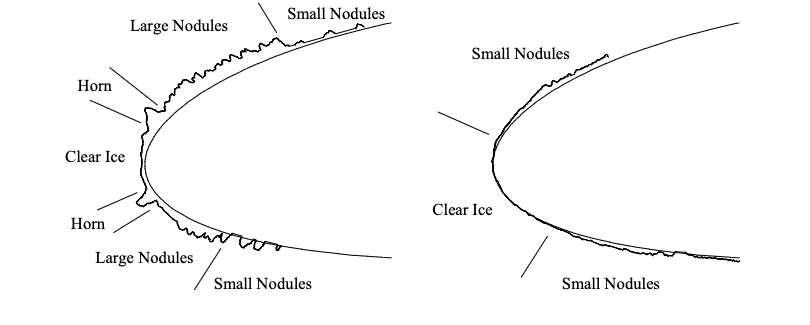
\includegraphics[width=.75\textwidth]{FIGURES/SLD/SLD_SHAPES.png}
\caption{Main features of SLD ice accretion \cite{whalen2005characteristics}.}
\label{fig:SLD_SHAPES}
\end{figure}

SLD behavior differs significantly from that of supercooled standard droplets. Because of their larger diameter, SLDs have greater inertia and their trajectories deviate more strongly from the airflow streamlines. Wright et al. \cite{wright2004semi} classified SLD effects according to their relative importance for aircraft icing simulations.

\subsection{Third-Order Effects}

Third-order SLD effects are generally small and are often neglected in practical icing simulations. This assumption is consistent with the hypotheses adopted in Section~\ref{sec:LagDropTracking}. These effects include the following:

\begin{itemize}
\item \textbf{Basset force:} This force accounts for the time history of the drag force. It is generally negligible when the viscosity of the carrier fluid is much smaller than that of the particles, as is the case for water droplets in air;
\item \textbf{Saffman force:} This lift force can be relevant for small particles in shear flows, but is typically more important for gas bubbles than for water droplets in icing applications;
\item \textbf{Turbulence effects:} Bhargava et al. \cite{bhargava2005numerical} investigated turbulence effects on droplet motion in the NASA IRT and found that they are generally of secondary importance, except in specific high-speed configurations such as rotor blades or propellers.
\end{itemize}

\subsection{Second-Order Effects: Deformation and Breakup}

Unlike standard droplets, SLDs may deform significantly as they travel through the flow field. Because of their larger diameter, they are more sensitive to aerodynamic pressure differences across the droplet surface. When the aerodynamic forces exceed the restoring effects of surface tension and viscosity, the assumption of spherical droplets becomes invalid.

Droplet deformation changes the effective drag coefficient and can therefore influence the droplet trajectory and the resulting impingement distribution. In more extreme cases, droplets may break up into smaller fragments, further modifying the droplet-size distribution and the water collection on the surface. However, except for some freezing-drizzle conditions, the influence of deformation and breakup appears to remain limited in many icing applications \cite{trontin2016revisited}.

\begin{figure}[htp]
\centering
\subfloat[Droplet deformation \cite{guido2011shear}]{%
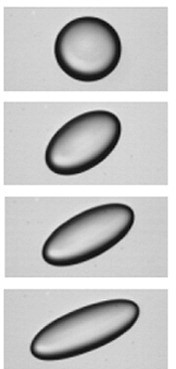
\includegraphics[width=0.15\textwidth]{FIGURES/SLD/dropletDeformation.jpg}%
\label{fig:deformation}%
}%
\hspace{2cm}%
\subfloat[Droplet breakup \cite{xu_wang_che_2022}]{%
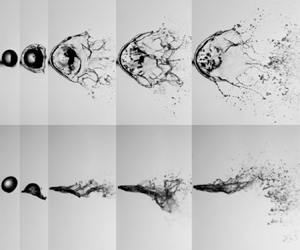
\includegraphics[width=0.37\textwidth]{FIGURES/SLD/dropletBreakup.png}%
\label{fig:dropletBreakup}%
}%
\caption{Examples of second-order SLD effects.}
\label{fig:SLD2ndOrder}
\end{figure}

\subsection{First-Order Effects: Sticking, Splashing, and Bouncing}

Droplet-wall interaction is one of the most important aspects of SLD modeling. When large droplets impact a surface, they do not necessarily stick completely. Depending on the impact conditions and surface properties, they may spread, bounce, splash, or generate secondary droplets. Experiments have shown that large droplets may fragment after impact, producing secondary droplets that can reimpinge farther downstream \cite{cossali1999impact,rein1993phenomena,alzaili2011experimental,vanzante2007database}. This mechanism increases the effective impingement limits compared with standard droplets.

The outcome of droplet impact depends on several parameters, including droplet diameter, impact velocity, impact angle, density, viscosity, surface tension, surface roughness, wettability, and wall temperature. These quantities are commonly expressed using nondimensional groups such as the Reynolds, Weber, and Ohnesorge numbers. The main droplet-wall interaction regimes can be summarized as follows \cite{trontin2017description}:

\begin{itemize}
\item \textbf{Sticking:} The droplet adheres to the wall, and no mass loss occurs. This regime is generally associated with low impact velocity;
\item \textbf{Bouncing:} A thin air film remains trapped between the droplet and the surface, preventing direct contact and causing the droplet to rebound;
\item \textbf{Deposition and spreading:} The droplet spreads along the surface, contributing to a liquid film or merging with an existing water film. Part of the kinetic energy is dissipated by viscous effects, while another part is converted into surface energy;
\item \textbf{Splashing:} At sufficiently high impact energy, viscous forces and surface tension are no longer able to maintain droplet integrity. The droplet fragments into secondary droplets, some of which are ejected from the surface.
\end{itemize}

\begin{figure}[htp]
\centering
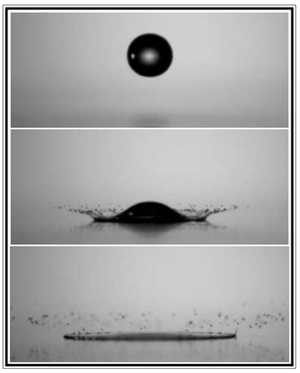
\includegraphics[width=.25\textwidth]{FIGURES/SLD/dropletSplashing.png}
\caption{Example of droplet splashing \cite{ball_what_2014}.}
\label{fig:splashing}
\end{figure}

Direct numerical simulation of droplet impact can be performed using interface-resolved methods such as the Volume of Fluid method \cite{hirt1981volume} or Moment of Fluid methods \cite{lian2014numerical}. However, such approaches require high-resolution meshes around each droplet and are therefore not practical for aircraft icing simulations involving millions of droplets. As a result, current SLD models generally rely on semi-empirical formulations calibrated against experimental data.

These models often introduce a mass-loss coefficient $f_m$, or equivalently a sticking efficiency $\epsilon$, to account for the fraction of droplet mass retained after impact. The corrected collection efficiency is then written as

\begin{equation}
\beta_{final} =(1.0 - f_m) , \beta_{0},
\end{equation}

or equivalently,

\begin{equation}
\beta_{final} = \epsilon, \beta_{0}.
\end{equation}

This correction can be applied as a post-processing step for both Eulerian and Lagrangian droplet models. However, secondary droplet reimpingement is more naturally handled in a Lagrangian framework. In this case, semi-empirical models can provide post-impact quantities, such as secondary droplet diameter and velocity, allowing the droplets to be reinjected into the computational domain.

In an Eulerian framework, secondary reimpingement is more difficult to model. One possible approach consists in modifying the boundary conditions on splashing surfaces \cite{bilodeau2016numerical}. The simulation is then performed in two stages. First, the original collection efficiency is computed and the splashing regions are identified. Second, selected wall faces are converted into inflow boundaries to model the reemission of secondary droplets. The final collection efficiency is then obtained as

\begin{equation}
\beta_{final} = \epsilon, \beta_{0} + \sum \beta_{re-impingement}.
\end{equation}

For complex three-dimensional geometries, however, the number of surface elements involved in reinjection may become very large, reducing the practical efficiency of this approach. Recent work has proposed converting all relevant boundary faces into inflow boundaries to reduce the computational cost \cite{capizzano2023extending}. Other approaches use statistical clustering to reduce the number of reinjection simulations \cite{bilodeau2016numerical}.

Table~\ref{tab:splashing_Models} summarizes several splashing models available in the literature. Mundo et al. \cite{mundo1998modeling} proposed one of the first semi-empirical models for droplet splashing, in which the mass-loss coefficient is related to the number and size distribution of secondary droplets. Trujillo et al. \cite{trujillo2000modelling} introduced a model based on the parameters proposed by Yarin and Weiss \cite{yarin1995impact}, including effects of droplet-generator frequency and surface roughness. Honsek et al. \cite{honsek2006fensap} later modified Trujillo’s formulation and implemented it in FENSAP-ICE.

Wright et al. \cite{wright2004semi} introduced the impact angle into the splashing parameters and mass-loss formulation. This makes splashing less likely for droplets impacting nearly normal to the surface and more likely near the impingement limits. Their model was calibrated by comparing computed water collection efficiencies with experimental data. Trontin et al. \cite{trontin2016revisited} proposed an alternative formulation based on subfunctions describing the dependence of mass loss on impact angle and kinetic energy. The model parameters were adjusted using comparisons with experimental data.

% Please add the following required packages to your document preamble:
% \usepackage{multirow}
\begin{table}[htb!]
\centering
\caption{SLD Splashing Models}
\label{tab:splashing_Models}
\begin{tabular}{ccc}
\hline
Source &
Mass Loss Coefficient &
Splashing Criterion \\ \hline\hline
\\
Mundo et al. \cite{mundo1998modeling} &
$n_s (\frac{d_s}{d_0})^3$ &
$K_M = (Oh^{-0.4}We)^{0.625} > 57.7$ \\ \\

\\
Trujillo et al. \cite{trujillo2000modelling} &
$0.8 [1.0 - e^{-0.85(K_y - 17)}]$ &
$K_y = \frac{1}{0.45^\frac{3}{8}}(Oh^{-0.4}We)^{0.3125} > 17$ \\ \\

\\
Honsek et al. \cite{honsek2006fensap} &
$\frac{3.8}{K_y^{0.5}} [1.0 - e^{-0.85(K_y - 17)}]$ &
$K_y > 17$ \\ \\

\\
Wright et al. \cite{wright2004semi} &
$0.7 (1.0 - sin(\theta_0)) [1.0-e^{-0.0092(K_M - 200.0)}]$ &
$\frac{0.859 \, K_m^{0.5} \, (\frac{\rho_{w}}{LWC})^{0.125}}{sin(\theta_0)^{1.25}} > 200.0$ \& $\theta < \frac{\pi}{2}$ \\ \\

\\
Trontin et al. \cite{trontin2016revisited} &
$1.0 - g(\frac{\theta}{\theta_c})f(\frac{K_c-K_0}{K_0})$ &
$ K_c = We_n \cdot Oh^{\frac{-2}{5}} > 657 $\\ \\
\hline
\end{tabular}
\end{table}


\section{Immersed-Boundary Methods}

The robustness of aircraft icing simulations is strongly affected by the geometry and mesh-update stages. In classical body-fitted approaches, the computational mesh must conform to the aircraft surface and must be regenerated or deformed after each ice accretion layer. As the ice shape grows, the geometry can become increasingly complex, making it difficult to maintain high-quality near-wall cells and avoid mesh failure. This issue is especially critical for three-dimensional multilayer simulations.

Immersed-boundary methods provide an alternative approach in which the geometry is represented independently of the computational mesh. The solid boundary may cut through grid cells, and boundary conditions are imposed through modifications of the governing equations or their discretization. This strategy can simplify mesh generation and improve robustness for complex and evolving geometries. However, each immersed-boundary formulation introduces specific numerical challenges related to accuracy, conservation, stability, wall modeling, and geometry representation.

\subsection{Classification}

Following the classification of Sotiropoulos and Yang \cite{sotiropoulos2014immersed}, immersed-boundary methods can be grouped into three main families: geometrical methods, continuous-forcing methods, and discrete-forcing methods. Geometrical methods modify the mesh or control volumes near the interface. Continuous-forcing methods add source terms to the governing equations to represent the boundary. Discrete-forcing methods impose the boundary conditions directly at the discrete level. The following sections summarize these approaches. Table~\ref{tab:IBM_MODELS} provides a comparison based on implementation complexity, accuracy, stability, and computational cost.

\subsubsection{Geometrical Methods}

Geometrical immersed-boundary methods rely on the ability of the solver to handle arbitrary cell shapes. These methods were introduced by Clarke et al. \cite{clarke1986euler} for Euler-flow simulations around multi-element airfoils. In this approach, a preprocessing step cuts the cells intersected by the solid boundary, as illustrated in Figure~\ref{fig:cutCell}. The resulting cut cells conform locally to the immersed interface.

\begin{figure}[htp]
\centering
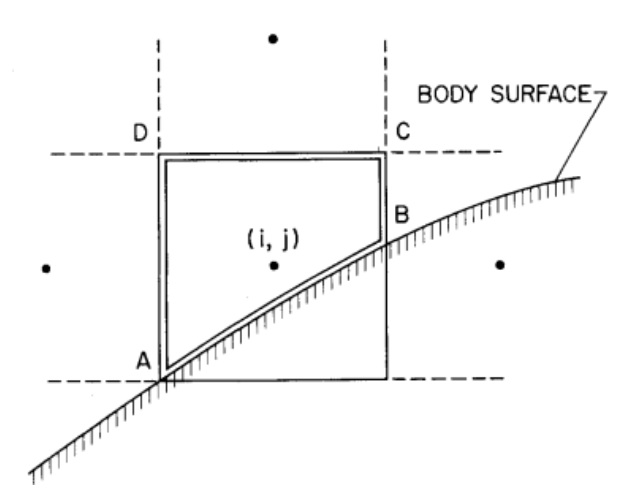
\includegraphics[width=.5\textwidth]{FIGURES/IBM/cutCell.png}
\caption{Boundary cut-cell method \cite{clarke1986euler}.}
\label{fig:cutCell}
\end{figure}

The main advantage of cut-cell methods is their sharp and conservative treatment of the boundary. In addition, the governing equations and numerical fluxes can often be kept close to those of the original solver. However, the geometric preprocessing is complex, particularly in three dimensions. Another major difficulty is the presence of very small cut cells, which can impose severe time-step restrictions and affect stability. Several remedies have been proposed, including cell merging \cite{glimm2003conservative}, cell linking \cite{kirkpatrick2003representation}, and cell mixing \cite{meyer2010conservative}.

\subsubsection{Continuous-Forcing Methods}

Continuous-forcing immersed-boundary methods modify the governing equations by adding a forcing term that accounts for the presence of the boundary. A generic system can be written as

\begin{equation}
\frac{\partial \boldsymbol{W}}{\partial t} = \boldsymbol{R} + \boldsymbol{F},
\label{eq:contForcing}
\end{equation}

where $\boldsymbol{W}$ represents the conservative variables, $\boldsymbol{R}$ is the residual of the original governing equations, and $\boldsymbol{F}$ is the immersed-boundary forcing term.

This class of methods originates from the work of Peskin \cite{peskin1972flow}, who introduced an immersed-boundary formulation for elastic boundaries in heart-flow simulations. In this method, the boundary is represented by Lagrangian markers located at positions $\boldsymbol{X}_k$ and moving with the fluid. The force is distributed to the surrounding grid points using a regularized Dirac function:

\begin{equation}
\boldsymbol{F} = \sum_k \boldsymbol{F}_k(t) \delta(\boldsymbol{r}_k),
\end{equation}

with

\begin{equation}
\boldsymbol{r}_k = \rvert \boldsymbol{x} - \boldsymbol{X}_k \rvert.
\end{equation}

Here, $\boldsymbol{F}k(t)$ is the force associated with marker $k$, typically obtained from a constitutive law. For rigid-body applications, the boundary can be modeled as a very stiff elastic structure. Lai and Peskin \cite{lai2000immersed} used a spring analogy in which the marker is forced toward an equilibrium position $\boldsymbol{X}{k,e}$:

\begin{equation}
\boldsymbol{F}_k(t) = k (\boldsymbol{X}k - \boldsymbol{X}{k,e}).
\label{eq:contForcingRigid}
\end{equation}

A high stiffness $k$ is required to mimic a rigid boundary, but this also makes the governing equations stiff and can lead to numerical instability. Implicit or semi-implicit treatments are therefore often required. Moreover, because the force is distributed over several grid points, the interface is diffuse, which generally limits the spatial accuracy of the method near the boundary.

Penalization methods provide another continuous-forcing strategy. The solid region is treated as a porous medium with very low permeability. This approach was introduced by Arquis and Caltagirone \cite{arquis1984conditions}. A source term is added to the momentum equations to drive the velocity inside the solid toward the solid velocity $\boldsymbol{u}_s$:

\begin{equation}
\boldsymbol{F} = \sum_i \lambda \chi_{s,i}(\boldsymbol{u}_{s,i} - \boldsymbol{u}),
\label{eq:contForcingPenal}
\end{equation}

where $\chi$ is a mask function identifying the solid region and $\lambda$ is a large penalization parameter. As for stiff elastic forcing, large values of $\lambda$ increase the stiffness of the equations and may require implicit or semi-implicit time integration.

\subsubsection{Discrete-Forcing Methods}

Discrete-forcing methods impose the immersed-boundary conditions directly in the discretized equations rather than modifying the continuous governing equations. Direct forcing, introduced by Mohd-Yusof \cite{mohd1997simulations}, is a representative example. For the incompressible Navier-Stokes equations, the momentum equation can be written as

\begin{equation}
\frac{\partial \boldsymbol{u}}{\partial t} = - \boldsymbol{u} \cdot \nabla \boldsymbol{u} - \nabla P + \frac{1}{Re} \nabla^2 \boldsymbol{u} + \boldsymbol{f},
\end{equation}

where $\boldsymbol{f}$ is the forcing term. Using an explicit Euler discretization gives

\begin{equation}
\frac{\boldsymbol{u}^{n+1} - \boldsymbol{u}^{n}}{\Delta t} = - \boldsymbol{u} \cdot \nabla \boldsymbol{u} - \nabla P + \frac{1}{Re} \nabla^2 \boldsymbol{u} + \boldsymbol{f}.
\end{equation}

The forcing term can then be selected to impose a target boundary velocity $\boldsymbol{u}_{target}$:

\begin{equation}
\boldsymbol{f} = \boldsymbol{u} \cdot \nabla \boldsymbol{u} + \nabla P - \frac{1}{Re} \nabla^2 \boldsymbol{u} + \frac{1}{\Delta t} (\boldsymbol{u}_{target} - \boldsymbol{u}^n).
\label{eq:discreteForcing}
\end{equation}

If the immersed boundary coincides with a cell center, the target value can be imposed exactly. In practice, this alignment is rare, and interpolation is required to avoid a staircase representation of the boundary. Unlike continuous-forcing methods, discrete-forcing methods do not introduce large source terms into the continuous equations and therefore avoid some stiffness-related stability issues. However, care is required near highly curved boundaries and at high Reynolds numbers, where internal flow structures inside the solid region may affect stability.

Ghost-cell methods are another widely used discrete-forcing approach \cite{mittal2008versatile}. In these methods, cells located inside the solid but adjacent to the fluid are identified as ghost cells. For each ghost cell, an image point is constructed in the fluid, usually by casting a ray normal to the interface from the ghost-cell center. Flow variables are interpolated at the image point from neighboring fluid cells, and the ghost-cell values are then assigned so that the desired boundary condition is satisfied at the immersed interface. Figure~\ref{fig:ghostCell} illustrates the construction of ghost cells and image points.

\begin{figure}[htp]
\centering
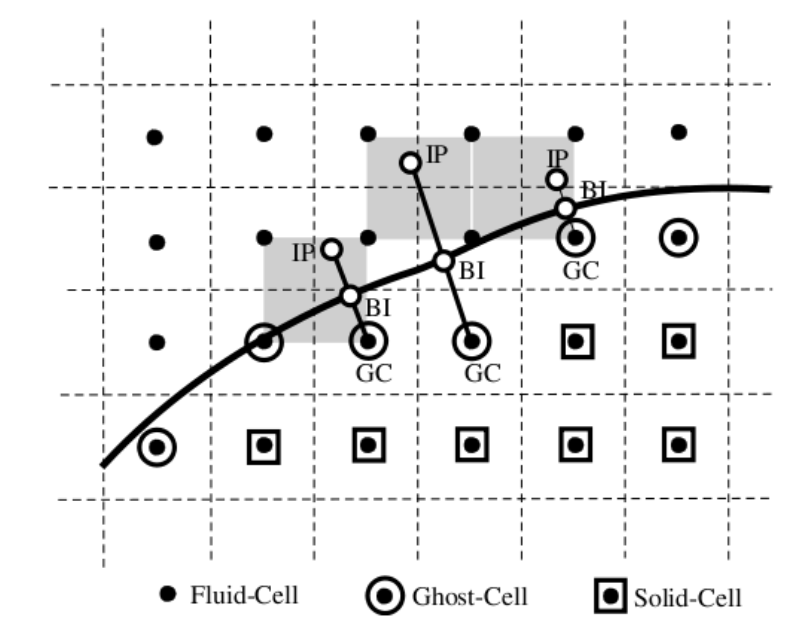
\includegraphics[width=.5\textwidth]{FIGURES/IBM/ghostCell.png}
\caption{Image-point and ghost-cell construction near an immersed boundary \cite{mittal2008versatile}.}
\label{fig:ghostCell}
\end{figure}

Ghost-cell methods can achieve first- or second-order spatial accuracy, depending on the interpolation strategy and the placement of the image point \cite{tseng2003ghost}. They also preserve the original form of the governing equations in the fluid region, which makes them attractive for compressible-flow solvers.

Face-forcing methods impose the boundary condition through modified fluxes at cell faces. This approach has been applied to Euler flows \cite{capizzano2007compressible}, RANS simulations \cite{capizzano2011turbulent}, and Eulerian droplet tracking \cite{capizzano2014eulerian}. The construction is similar to the ghost-cell approach, but the image point is defined along a normal passing through the cell face rather than the ghost-cell center. The reconstructed state is then used to compute the flux through the immersed boundary face.

\begin{figure}[htp]
\centering
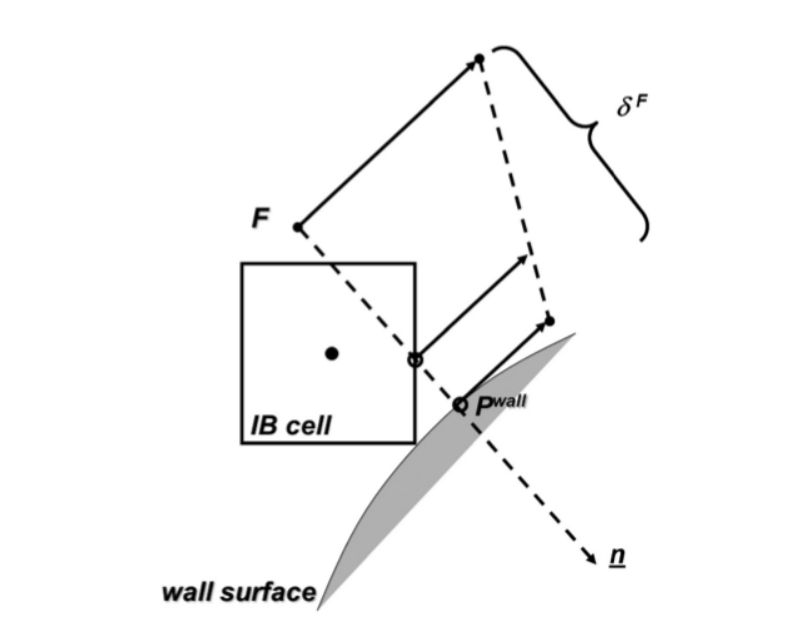
\includegraphics[width=.5\textwidth]{FIGURES/IBM/faceForcing.png}
\caption{Illustration of face forcing near an immersed boundary \cite{capizzano2014eulerian}.}
\label{fig:faceForcing}
\end{figure}

% Please add the following required packages to your document preamble:
% \usepackage{multirow}

\begin{table}[htp!]
\centering
\caption{IBM Comparison}
\label{tab:IBM_MODELS}
\begin{tabular}{ccccccc}
\hline
Class & Method & Implementation & Accuracy & Stability
 & Cost \\
\hline
\hline
\\

Geometrical & Cut-Cell & Hard & $1^{st}$ & Hard & High \\

\\

\multirow{3}{*}{Continuous Forcing} & Rigid Body Forcing & Easy & $1^{st}$ Order & Hard & Low \\ \\

& Penalization & Easy & $2^{nd}$ Order & Hard & Low \\

\\

\multirow{5}{*}{Discrete Forcing} & Direct Forcing & Medium & $2^{nd}$ Order & Hard & Low  \\ \\
& Ghost-Cell & Medium & $2^{nd}$ Order  & No Issues  & High \\ \\
& Face Forcing & Medium & $2^{nd}$ Order & No Issues & High \\ \\ 
\hline
\end{tabular}
\end{table}


\subsection{Surface Representation}

Surface representation is an essential component of both ice accretion simulations and immersed-boundary methods. In ice accretion, the surface must be updated as ice grows. In immersed-boundary methods, the interface must be located accurately in order to impose boundary conditions and compute quantities such as normals, wall distances, and curvature.

Two main categories of interface representation exist in the literature: interface tracking and interface capturing. Interface-tracking methods represent the surface explicitly using markers or mesh points that move with the interface. Interface-capturing methods represent the surface implicitly as a field defined over the computational domain.

\subsubsection{Interface Tracking}

Interface-tracking methods are commonly used for problems involving discontinuous interfaces, such as two-phase flows. The interface is represented by marker points distributed either directly on the interface or within control volumes. Examples include the Marker-and-Cell and Particle-in-Cell methods.

The main advantage of interface tracking is that the interface position is explicitly known, which enables an accurate representation of fine surface structures. However, because the interface markers do not generally coincide with the computational grid, flow quantities must be interpolated from the grid to the markers. This interpolation may introduce errors. In addition, large interface deformations can lead to poor marker distribution, requiring reseeding or remeshing. Topological changes, such as merging or breakup, are also difficult to handle robustly with explicit interface tracking.

\subsubsection{Interface Capturing}

Interface-capturing methods represent the interface implicitly using a field variable. One of the most common approaches is the level-set method. In this method, the interface is represented as the zero contour of a scalar function $\phi$ defined over the computational domain \cite{sethian2003level}. The level-set function is advected according to

\begin{equation}
\frac{\partial \phi }{\partial t} + \boldsymbol{V} \cdot \nabla \phi = \phi (\nabla \cdot \boldsymbol{V}),
\label{eq:levelSet}
\end{equation}

where $\boldsymbol{V}$ is the interface velocity field. The function $\phi$ is commonly defined as positive in the fluid, negative in the solid, and zero at the interface. When $\phi$ is a signed-distance function, interface normals and curvature can be obtained from

\begin{equation}
\boldsymbol{n} = \frac{\nabla \phi}{\rvert \nabla \phi \rvert},
\end{equation}

and

\begin{equation}
\boldsymbol{\kappa} = \nabla \cdot \frac{\nabla \phi}{\rvert \nabla \phi \rvert}.
\end{equation}

This information is useful for immersed-boundary methods, geometry evolution, and turbulence modeling.

Level-set methods can naturally handle topological changes and provide smooth interface normals. However, they are not strictly conservative. In addition, during advection, the signed-distance property may be lost, especially when tangential velocity components are present near the interface. A reinitialization or redistancing procedure is therefore often required to restore the signed-distance property. The interface velocity must also be known not only at the interface but in its neighborhood, which may require an additional velocity-extension step.

Another widely used interface-capturing technique is the Volume of Fluid method. In this approach, a volume fraction $f(\boldsymbol{x},t)$ is used to represent the fraction of a given material contained in each cell \cite{rauschenberger2013comparative}:

\begin{equation}
f(\boldsymbol{x},t) =
\begin{cases}
0 & \text{fluid},\\
[0,1] & \text{interface},\\
1 & \text{solid}.
\end{cases}
\end{equation}

The interface is reconstructed from the volume fraction in each mixed cell. The accuracy of the method depends strongly on the reconstruction strategy. The Simple Linear Interface Calculation method is first-order accurate, whereas the Piecewise Linear Interface Calculation method can achieve second-order accuracy.

The VoF/PLIC algorithm is generally divided into two steps: reconstruction and propagation. Figure~\ref{fig:VOF} illustrates the reconstruction process for SLIC and PLIC. PLIC is usually preferred because it provides a more accurate representation of the interface. However, for highly curved interfaces, features smaller than the local grid size cannot be resolved \cite{scardovelli1999direct}.

\begin{figure}[htp]
\centering
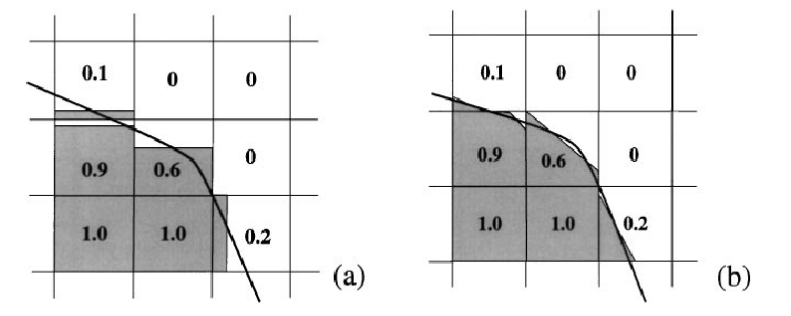
\includegraphics[width=.75\textwidth]{FIGURES/IBM/VOF.png}
\caption{Interface reconstruction using (a) SLIC and (b) PLIC \cite{scardovelli1999direct}.}
\label{fig:VOF}
\end{figure}

Hybrid methods combining level-set and VoF approaches have also been proposed. The Coupled Level Set Volume-of-Fluid method, introduced by Marter \cite{marter2017methode}, combines the smooth geometric information of the level-set method with the conservation properties of VoF. In this approach, both fields are evolved simultaneously. The VoF field maintains conservation, while the level-set field provides normals, curvature, and distance information. The level-set interface is corrected using the VoF field, and a redistancing step is performed to maintain the signed-distance property.

The main limitation of CLSVOF methods is their implementation complexity and computational cost, since both the level-set and VoF equations must be solved and coupled. Nevertheless, they provide improved capabilities compared with either method used alone.

\subsection{Wall Functions}\label{sec:wallFunctions}

At high Reynolds numbers, mean-flow gradients near the wall become very steep. In low-Reynolds-number RANS approaches, the turbulence model is integrated all the way to the wall. This requires very fine near-wall meshes and imposes strong constraints on the first-cell height, orthogonality, and grid smoothness. In ice accretion simulations, these constraints are particularly difficult to maintain because the surface evolves and may develop complex features such as horns, scallops, and runback ice.

Wall functions provide a practical alternative by using semi-analytical near-wall profiles for velocity and temperature. Instead of resolving the entire viscous sublayer, wall functions model the relation between wall quantities and flow variables at a finite distance from the wall. This reduces mesh requirements and can improve the robustness of icing simulations, especially in immersed-boundary or multilayer frameworks.

Near the wall, streamwise gradients are often small compared with wall-normal gradients. For an incompressible steady flow, the RANS momentum equation can be simplified as

\begin{equation}
\frac{d}{dy} \left((\mu + \mu_t) \frac{du}{dy}\right) = \frac{dp}{dx}.
\label{eq:reducedRANS}
\end{equation}

Assuming a zero pressure gradient and integrating once gives

\begin{equation}
(\mu + \mu_t) \frac{du}{dy}= \tau_w,
\label{eq:reducedRANSTau}
\end{equation}

where $\tau_w$ is the wall shear stress. In nondimensional form, this becomes

\begin{equation}
(1 + \nu_t^+) \frac{du^+}{dy^+}= 1.
\label{eq:reducedRANSTauND}
\end{equation}

The inner region of the boundary layer is commonly divided into three subregions:

\begin{itemize}
\item \textbf{Viscous sublayer} ($y^+ < 5$): viscous effects dominate and turbulent viscosity is negligible. The velocity profile is approximately linear, $u^+ = y^+$;
\item \textbf{Buffer layer} ($5 \leq y^+ < 30$): viscous and turbulent effects are both important;
\item \textbf{Logarithmic layer} ($y^+ \geq 30$): turbulent transport dominates. Assuming $\nu_t^+ = \kappa y^+$, where $\kappa \approx 0.41$ is the von Karman constant, the velocity profile follows the logarithmic law.
\end{itemize}

The standard wall function is therefore written as

\begin{equation}
u^+ =
\begin{cases}
y^+ & y^+ < 5,\\
\frac{1}{\kappa} \ln(y^+) + C & y^+ \geq 30,
\end{cases}
\label{eq:standardwallfunc}
\end{equation}

where $C$ is an empirical constant, typically between 5.0 and 5.5 depending on the turbulence model and calibration.

\begin{figure}[htp]
\centering
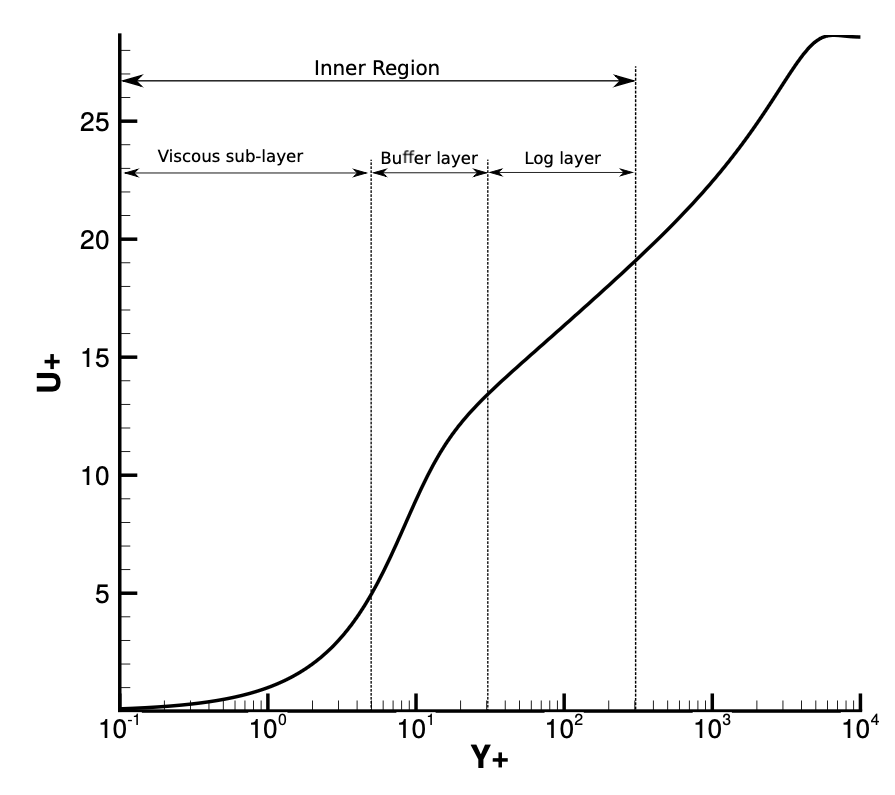
\includegraphics[width=.5\textwidth]{FIGURES/IBM/wallFunctions.png}
\caption{Illustration of the different layers of a turbulent boundary layer \cite{prakash2019rans}.}
\label{fig:BL}
\end{figure}

A similar analysis can be applied to the energy equation to obtain temperature wall functions. The simplified energy equation can be written as

\begin{equation}
\frac{d}{dy} \left[ \left( \frac{\mu}{Pr} + \frac{\mu_t}{Pr_t} \right) \frac{dT}{dy} \right ] = 0.
\label{eq:reducedEnergy}
\end{equation}

The corresponding nondimensional temperature profile is

\begin{equation}
T^+ =
\begin{cases}
Pr , y^+ & y^+ < 5,\\
\frac{Pr_t}{\kappa_T} \ln(y^+) + C_T & y^+ \geq 30,
\end{cases}
\label{eq:tempLayers}
\end{equation}

where $\kappa_T = 0.48$ and $C_T = 3.9$ are empirical constants \cite{kader1972heat}.

\subsubsection{Velocity Wall Functions}

Several velocity wall functions have been proposed in the literature. The simplest is the standard wall function given in Equation~\ref{eq:standardwallfunc}. However, the buffer layer is difficult to model analytically because both viscous and turbulent effects are important. This has motivated the development of more general wall laws that interpolate between the viscous sublayer and logarithmic region. Such formulations are often referred to as universal wall functions because they describe the entire inner region. Table~\ref{tab:veloctityprofiles} summarizes several commonly used velocity wall functions.

% Please add the following required packages to your document preamble:
% \usepackage{multirow}
\begin{table}[htb!]
\centering
\caption{Velocity Wall Functions}
\label{tab:veloctityprofiles}
\begin{tabular}{ccc}
\hline
Source &
SA or $k-\omega$ SST &
Velocity Profile \\ \hline\hline
\\
Spalding \cite{spalding1961single}  &
Both &
$y^+ = u^+ + e^{-\kappa B} (1 - e^{\kappa u^+} - \frac{(\kappa u^+)}{1!} - \frac{(\kappa u^+)^2}{2!} - ...)$ \\ \\

\\

Reichardt \cite{reichardt1951vollstandige} & Both & $u^+ = \frac{ln(1+\kappa y^+)}{\kappa} + 7.8 (1-e^{-\frac{y^+}{11}}-\frac{y^+}{11}e^{-\frac{y^+}{3}})$ \\ \\


\multirow{3}{*}{Knopp \cite{knopp2006grid}} & SA & $F_{SA,\alpha} =(1-\phi_{SA}) F_{Sp,5} +\phi_{SA}F_{Rei,m}$ with $\phi_{SA} = tanh[(\frac{y^+}{24})^3]$\\ \\

& $k-\omega$ SST & $F_{k\omega,\alpha} =(1-\phi_{k\omega}) F_{Sp,3} +\phi_{k\omega}F_{Rei,m}$ with $\phi_{k\omega} = tanh[(\frac{y^+}{50})^2]$\\ \\

\multirow{3}{*}{Allmaras \cite{allmaras2012modifications}} & \multirow{2}{*}{SA} & $u^+ = \Bar{B} + c_1ln((y^+ + a_1)^2 + b_1^2) - c_2ln((y^+ + a_2)^2 + b_2^2)$ \\ & & $- c_3 atan2(b_1,y^+ + a_1) - c_4atan2(b_2,y^+ + a_2)$ \\ \\ 
\hline
\end{tabular}
\end{table}


More general wall functions have also been developed for nonequilibrium boundary layers. Craft et al. \cite{craft2002progress} proposed an Analytical Wall Function that accounts for pressure-gradient and convection effects by integrating a more general near-wall momentum equation. This requires an assumed relation between turbulent viscosity and wall-normal distance.

Gant \cite{gant2002development} proposed a wall function based on the numerical integration of a parabolized transport equation on a one-dimensional subgrid. The subgrid solution is then interpolated to the first wall cell.

Popovac and Hanjalic \cite{popovac2007compound} observed that many advanced wall functions involve complex expressions that are difficult to implement in general-purpose CFD solvers. They proposed a simplified formulation based on a modified logarithmic law:

\begin{equation}
u^+ = \frac{1}{\psi \kappa} \ln(y^+) + C,
\label{eq:craft}
\end{equation}

where $\psi$ accounts for nonequilibrium effects. For equilibrium flows, $\psi=1$, and the standard logarithmic law is recovered. They also combined this generalized wall function with the mixing function proposed by Kader \cite{kader1972heat} to extend its validity throughout the inner region.

Kalitzin et al. \cite{kalitzin2005near} introduced a lookup-table wall function based on well-resolved Couette-flow simulations. In this approach, nondimensional profiles of velocity, temperature, and turbulence variables are precomputed and stored for later use.

\subsubsection{Temperature Wall Functions}

As for velocity, the standard temperature wall function given in Equation~\ref{eq:tempLayers} provides a simple representation of the near-wall thermal field. However, the buffer-layer behavior is difficult to describe using simple analytical expressions. Several temperature wall functions have therefore been proposed to provide continuous profiles across the inner region. Table~\ref{tab:temperatureprofiles} summarizes representative models.

The wall functions proposed by Craft et al. \cite{craft2002progress} and Popovac and Hanjalic \cite{popovac2007compound} include heat-transfer effects in addition to velocity profiles. Another strategy is to use lookup tables for isothermal walls, where variations of $T^+$ with $y^+$ are precomputed. These approaches have also been extended to include pressure-gradient effects, as shown by Lacombe et al. \cite{lacombe2019compatible}.

% Please add the following required packages to your document preamble:
% \usepackage{multirow}
\begin{table}[htb!]
\centering
\caption{Temperature Wall Functions}
\label{tab:temperatureprofiles}
\begin{tabular}{ccc}
\hline
Source &
SA or $k-\omega$ SST &
Temperature Profile\\ \hline\hline
\\
\multirow{3}{*}{Kader \cite{kader1972heat}} & \multirow{2}{*}{Both} & $\theta^+ = Pry^+ e^{-\tau} + 2.12 ln((1+y^+) + \beta(Pr)) e^{-\frac{1}{\tau}}$ \\ \\ & & $\tau = \frac{0.01 (Pry^+)^4}{1+5Pr^3y^+}$ , $\beta = (3.85 Pr^{\frac{1}{3}}-1.3)^2+ 2.12ln(Pr)$ \\ \\ 

\\

\multirow{3}{*}{Jayatillaka \cite{jayatilleke1966influence}} & \multirow{2}{*}{Both} & $T^+ = Pr_t(u^+ + P_f)$ \\ \\ & & $P_f = 0.24 [(\frac{Pr}{Pr_t})^\frac{3}{4}-1][1+0.28 exp(-0.007 \frac{Pr_t}{Pr})]$ \\ \\ 

\\


\multirow{3}{*}{Arpaci  \cite{arpaci1984heat}} & \multirow{2}{*}{Both} & $  T^+ =
    \begin{cases}
      Pr \, y^+ & y^+ < y^+_1\\
    a_2 - \frac{Pr_t}{2a_1(y^+)^2} & y^+_1 \leq y^+ < y^+_2  \\
    \frac{Pr_t}{\kappa} ln(y^+) + \beta &  y^+ \geq y^+_2 
    \end{cases} $ \\  \\ \\ 
\hline
\end{tabular}
\end{table}


\subsubsection{Influence of Roughness}

Surface roughness plays an important role in aircraft icing simulations. Roughness modifies the near-wall turbulence and can increase convective heat transfer, which directly affects the predicted ice shape. This is particularly important for glaze ice, where not all impinging water freezes immediately upon impact. Instead, a liquid film may run back from the stagnation region and freeze downstream, contributing to horn formation. In such cases, roughness is related to beads, rivulets, and irregular surface features that develop during ice accretion \cite{hansman1989investigation}.

The pioneering experiments of Nikuradse \cite{nikuradse1933laws} on sand-roughened pipes provided fundamental insight into rough-wall turbulent flows. One of the main observations was that roughness produces a downward shift of the logarithmic velocity profile, as illustrated in Figure~\ref{fig:BLShift}. The rough-wall logarithmic law can be written as

\begin{equation}
u^+ = \frac{1}{\kappa} \ln(y^+) + C - \Delta u^+,
\end{equation}

where $\Delta u^+$ is the roughness function.

\begin{figure}[htp]
\centering
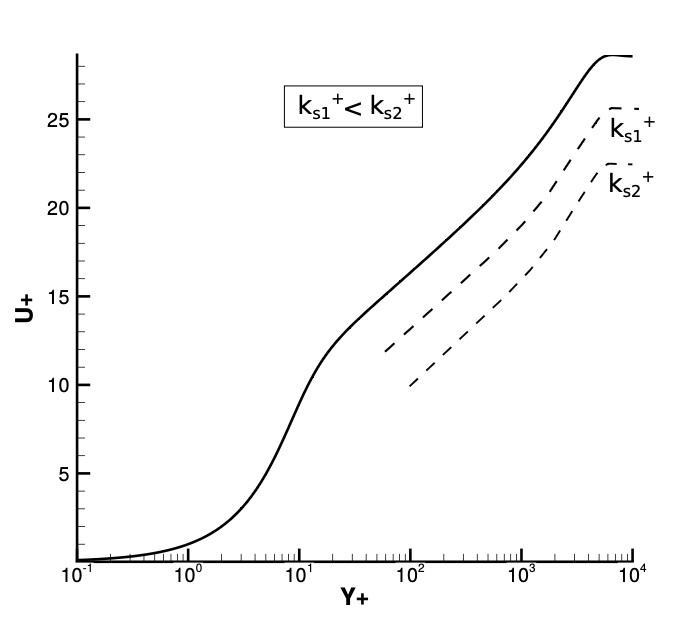
\includegraphics[width=.5\textwidth]{FIGURES/IBM/roughnessEffect.png}
\caption{Influence of roughness on the velocity profile \cite{prakash2019rans}.}
\label{fig:BLShift}
\end{figure}

Nikuradse classified roughness effects using the nondimensional roughness height. Schlichting \cite{schlichting1936experimentelle} later showed that a single geometric parameter is generally insufficient to describe the effect of arbitrary roughness elements. Roughness spacing, shape, inclination, and density can all influence the flow response. This led to the concept of equivalent sand-grain roughness $k_s$, defined as the roughness height that produces the same shift in the logarithmic velocity profile as the real surface. This parameter is widely used in modern CFD solvers.

Several wall-function extensions include roughness effects by introducing a shift in the velocity profile. As summarized by Prakash et al. \cite{prakash2019rans}, the rough-wall velocity profile can be related to the smooth-wall profile through

\begin{equation}
\frac{du_{rough}^+}{dy^+} (y^+) = \frac{du_{smooth}^+}{dy^+} (y^+ + y_0^+),
\end{equation}

\begin{equation}
u_{rough}^+ (y^+)= u_{smooth}^+(y^+ + y_0^+) - u_{smooth}^+(y_0^+),
\end{equation}

and

\begin{equation}
\Delta u^+ =  u_{smooth}^+(y_0^+).
\label{eq:roughnessExt}
\end{equation}

Here, $y_0^+$ is a wall shift related to the nondimensional roughness height $k_s^+$. Similar corrections can be applied to temperature wall functions.

The influence of roughness is commonly divided into three regimes:

\begin{itemize}
\item \textbf{Hydraulically smooth regime} ($k_s^+ < 5$): the roughness elements are contained within the viscous sublayer, and their effect on skin friction is small. The surface can be treated as smooth;
\item \textbf{Transitionally rough regime} ($5 \leq k_s^+ \leq 70$): roughness begins to affect the near-wall flow, the viscous sublayer is reduced, and skin friction increases. This regime is sensitive to roughness shape, spacing, and distribution;
\item \textbf{Fully rough regime} ($k_s^+ > 70$): the viscous sublayer is disrupted, and the skin-friction coefficient becomes largely independent of Reynolds number. The flow response is mainly controlled by the roughness geometry.
\end{itemize}

In aircraft icing simulations, roughness modeling remains a significant source of uncertainty. Since roughness affects heat transfer and water runback, it can strongly influence glaze-ice accretion and horn formation. A robust numerical framework must therefore account for roughness effects consistently within the flow, heat-transfer, and thermodynamic models.
